\chapter{Lag Compensation}
\label{sec:hla-lag}

In this chapter,
we present simulations which compensate for time lags introduced due to
HLA time management.
The lags appear when published data are sent from one federate to
its subscribers, and
it becomes particularly noticeable when data ownership is transferred
between federates.

There are two \TrickHLA\ mechanisms which allow simulation developers
to compensate for HLA-introduced lag:
publisher-side and subscriber-side compensation.

% -------------------------------------------------------------------------
\section{What is a Lag Compensator?}

% -----------------------------------
\subsection{The class {\tt TrickHLALagCompensation}}

\TrickHLA\ defines a C++ class which may be subclassed by simulation
developers in order to implement either kind of lag compensation.
The class header is shown below.

\begin{lstlisting}[caption={The {\tt TrickHLALagCompensation} class},label={list:TrickHLALagCompensation}]
class TrickHLALagCompensation
{
   friend class InputProcessor;
   friend void init_attrTrickHLALagCompensation();

  public:
   TrickHLALagCompensation() {};           // default constructor
   virtual ~TrickHLALagCompensation() {};  // destructor

   virtual void send_lag_compensation();   // RETURN: -- None.

   virtual void receive_lag_compensation() // RETURN: -- None.
};
\end{lstlisting}

To use this class,
simulation developers subclass it, overriding the relevant send/receive methods.
The \TrickHLA\ infrastructure automatically invokes those methods
for publishers and subscribers at the appropriate time.

Developers only need to be concerned with the algorithm defined in these
methods; the logistics of invoking them at the appropriate time is taken
handled by \TrickHLA.
The following subsections illustrate how this is done in the \simplesine
model.

% -----------------------------------
\subsection{Lag compensation in \simplesine}
% -------------
\subsubsection{\tt simplesine\_compensate()}

The \simplesine model includes a {\tt simplesine\_compensate()} function
which does most of the lag compensation work.
It is based on the equations~\ref{eq:analytic-equations}.
Using those equations, the state at time $t + \Delta t$ can be written as
\begin{subequations}
\label{eq:analytic-compensation-equations}
\begin{align}
x(t + \Delta t)       &= A        \sin {(\omega (t + \Delta t) + \phi)}, \\
\dot{x}(t + \Delta t) &= A \omega \cos {(\omega (t + \Delta t) + \phi)}.
\end{align}
\end{subequations}

With a bit of trignometry and rearranging, the compensated state at time
$t + \Delta t$ can be written in terms of the uncompensated state at time $t$
as follows.
\begin{subequations}
\label{eq:analytic-compensation-equations-2}
\begin{align}
x(t + \Delta t)
  &=
    x(t)       \cos {\omega \Delta t}
    +
    \frac{\dot{x}(t)}{\omega} \sin { \omega \Delta t}
  \\
\dot{x}(t + \Delta t)
  &=
    \dot{x}(t) \cos {\omega \Delta t}
    -
    x(t) \omega \sin { \omega \Delta t}
\end{align}
\end{subequations}

The compensate function is shown below.
It takes an uncompensated state and $\Delta t$ as inputs
and calculates the corresonded compensated state at time $t + \Delta t$.

\begin{lstlisting}[caption={The {\tt simplesine\_compensate} function},label={list:simplesine-compensate}]
void simplesine_compensate(
  simplesine_params_T* paramsP,
  simplesine_state_T* uncompensated_stateP,
  simplesine_state_T* compensated_stateP,
  double dt )
{
  const double w = paramsP->w;
  const double wdt = w * dt;
  const double sinwdt = sin( wdt );
  const double coswdt = cos( wdt );

  const double x     = uncompensated_stateP->x;
  const double x_dot = uncompensated_stateP->x_dot;

  // Calculate the compensated state.
  const double x_compensated     = x     * coswdt  +  x_dot * sinwdt / w ;
  const double x_dot_compensated = x_dot * coswdt  -  x     * sinwdt * w;

  // Save the compenstated state.
  compensated_stateP->x     = x_compensated;
  compensated_stateP->x_dot = x_dot_compensated;
}
\end{lstlisting}

% -------------
\subsubsection{\tt simplesine\_LagCompensation}

The simplesine subsclass of {\tt TrickHLALagCompensation} is shown below.
It relies on the {\tt simple\-sine\-\_comp\-ensate()} function to do the real work, transforming the uncompensated state pointed to by
{\tt uncompensated\_stateP}
into a transformed state pointed to by
{\tt compensated\_stateP}.
These two pointers are initialized by the {\tt initialize()} method,
which is unique to this class (i.e., not part of the interface defined by the
{\tt TrickHLALagCompensation} class).

\begin{lstlisting}[caption={The {\tt simplesine\_LagCompensation} class header},label={list:simplesine-LagCompensation-header}]
#include "simplesine.h"
#include "TrickHLA/include/TrickHLALagCompensation.hh"

class simplesine_LagCompensator : public TrickHLALagCompensation
{
  friend class InputProcessor;
  friend void init_attrsimplesine_LagCompensator();

  public:
   simplesine_LagCompensator();
   virtual ~simplesine_LagCompensator();

   int initialize( simplesine_T* sim_dataP, simplesine_T* lag_comp_dataP );
   virtual void send_lag_compensation();
   virtual void receive_lag_compensation();

  private:
    simplesine_T* uncompensated_stateP;
    simplesine_T* compensated_stateP;
};
\end{lstlisting}

\begin{lstlisting}[caption={The {\tt simplesine\_LagCompensation} class methods},label={list:simplesine-LagCompensation-methods}]
/********************************* TRICK HEADER *******************************
PURPOSE: (This class provides lag compensation.)
LIBRARY DEPENDENCY: ((simplesine_compensate.o))
*******************************************************************************/
// System include files.
#include <math.h>
#include <stdlib.h>
#include <iostream>
#include <string>

using namespace std;

#include "sim_services/include/exec_proto.h"
#include "trick_utils/math/include/trick_math.h"

#include "../include/simplesine_proto.h"
#include "../include/simplesine_LagCompensator.hh"

/* ---------------------------------------------------------------------------
PURPOSE: (Default constructor for the sine wave lag compensation.)
------------------------------------------------------------------------------*/
simplesine_LagCompensator::simplesine_LagCompensator() // RETURN: -- None.
{ }

/* ---------------------------------------------------------------------------
PURPOSE: (Frees memory allocated.)
------------------------------------------------------------------------------*/
simplesine_LagCompensator::~simplesine_LagCompensator() // RETURN: -- None.
{ }

/* ---------------------------------------------------------------------------
PURPOSE: (Initializes the Sine Lag Compensation.)
------------------------------------------------------------------------------*/
int simplesine_LagCompensator::initialize( // RETURN: -- Always returns zero.
      simplesine_T * uncompensated_stateP, // IN:     -- Simulation data.
      simplesine_T * compensated_stateP )  // IN:     -- Lag Compensation data.
{
   this->uncompensated_stateP = uncompensated_stateP;
   this->compensated_stateP = compensated_stateP;
   return( 0 );
}

/* ---------------------------------------------------------------------------
PURPOSE: (Send-side lag-compensation where we propagate the sine wave
  state head by dt to predict the value at the next data cycle.)
------------------------------------------------------------------------------*/
void simplesine_LagCompensator::send_lag_compensation() // RETURN: -- None.
{
   double dt = get_fed_lookahead().getDoubleTime();

   simplesine_compensate( &(uncompensated_stateP->params),
                          &(uncompensated_stateP->state),
                          &(compensated_stateP->state),
                          dt );
}

/* ---------------------------------------------------------------------------
PURPOSE: (Receiveside lag-compensation where we propagate the sine wave
  state ahead by dt to predict the value at the next data cycle.)
------------------------------------------------------------------------------*/
void simplesine_LagCompensator::receive_lag_compensation() // RETURN: -- None.
{
   double dt = get_fed_lookahead().getDoubleTime();

   simplesine_compensate( &(uncompensated_stateP->params),
                          &(uncompensated_stateP->state),
                          &(compensated_stateP->state),
                          dt );
}
\end{lstlisting}


% -------------------------------------------------------------------------
\section{Publisher-resident Compensation}

This approach to lag compensation is handled by the publisher of data before
it is sent out via HLA.
Since the compensation is performed by the publisher, subscribers need not
implement any lag-related logic.
This section demonstrates how to implement kind of lag compensation.

% -----------------------------------
\subsection{{\tt SIM\_simplesine\_hla\_pub\_lagComp}}

Implementing publisher-side lag compensation in an existing (non-compensating)
\TrickHLA\ simulation is very easy.
This simulation illustrates what is required.
It is based on the {\tt SIM\_simplesine\_hla\_pub} simulation and differs
only in that the {\tt publisher} sim object has a few new elements.

The sim object is shown in Listing~\ref{list:pub-lag-sim-object}.
The main differences between this simulation's \sdefine and that of the
publisher discussed in Chapter~\ref{sec:hla-pubsub} are
\begin{itemize}
\item{
  the declaration of two \simplesine variables,
  one for uncompensated data and the other for compensated,
}
\item{
  the declaration of a {\em lag compensator} variable, and
}
\item{
  the initialization job for the lag compensator
}
\end{itemize}

\begin{lstlisting}[caption={{\tt publisher} sim object for publisher-side lag compensation},label={list:pub-lag-sim-object}]
sim_object
{
  simplesine: simplesine_T uncompensated_simplesine (simplesine/data/simplesine.d);
  simplesine: simplesine_T compensated_simplesine (simplesine/data/simplesine.d);
  simplesine: simplesine_LagCompensator lag_compensator;

  (initialization) simplesine:
    simplesine_calc(
      simplesine_T* P = &publisher.uncompensated_simplesine,
      double t = sys.exec.out.time );

  (initialization) simplesine:
    publisher.lag_compensator.initialize(
      simplesine_T* uncompensatedP = &publisher.uncompensated_simplesine,
      simplesine_T* compensatedP = &publisher.compensated_simplesine );

  (PROPAGATE_TIMESTEP, scheduled) simplesine:
    simplesine_calc(
      simplesine_T* P = &publisher.uncompensated_simplesine,
      double t = sys.exec.out.time );
} publisher ;
\end{lstlisting}

% -----------------------------------
\subsection{Input file}

The input file for the lag compensating publisher is virtually identical
to the non-compensating publisher discussed previously with the following
exceptions.
\begin{itemize}
\item{
  The lag compensator defined in the \sdefine file is explicitly
  associated with the object being published and in particular is
  specified as a publisher-resident (sending) compensator by adding
  the following two lines to the input file:
  \begin{verbatim}
THLA.manager.objects[0].lag_comp      = &publisher.lag_compensator;
THLA.manager.objects[0].lag_comp_type = THLA_LAG_COMP_SEND_SIDE;
  \end{verbatim}
}
\item{
  Since the \sdefine for the compensating publisher now includes
  two \simplesine variables,
  one uncompensated and the other compensated,
  the lines in the input file which specify the Trick variable names
  to publish are changed accordingly from
  {\tt publisher.simplesine} to
  {\tt publisher.compensated\_simplesine}.
}
\end{itemize}

% -----------------------------------
\subsection{Output}

In this section,
we show the results of running a subscriber,
{\tt SIM\_simplesine\_hla\_sub}
along with the lag-compensating
publisher,
{\tt SIM\_simplesine\_hla\_pub\_lagComp}.

Unlike Figure~\ref{fig:hla-sub-output} on page~\pageref{fig:hla-sub-output},
where the subscriber is seen to be 1sec out of phase with the true state,
when the subscriber received {\em lag compensated} data from the publisher,
the subscriber's sine wave is in phase with the publisher
as shown in Figure~\ref{fig:hla-pub-lagComp-output}.
The error plot on this graph closely resembles the error plot of
Figure~\ref{fig:SIM-pubsub-input} on page~\pageref{fig:SIM-pubsub-input},
in which the publisher and subscriber are resident
in the same simulation, showing that the publisher's lag compensation
removes the HLA-induced lag.

\begin{figure}[h]
  \begin{center}
    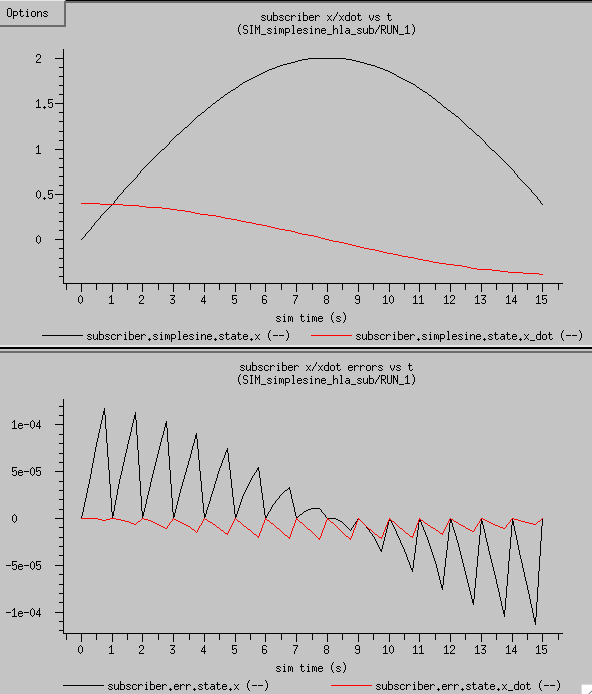
\includegraphics[width=4.5in]{TrickHLAUser-SIM-hla-pub-lagComp.png}
  \end{center}
\caption{Output from {\tt SIM\_simplesine\_hla\_pub\_lagComp}}
\label{fig:hla-pub-lagComp-output}
\end{figure}

\clearpage

% -------------------------------------------------------------------------
\section{Subscriber-resident Compensation}

This approach to lag compensation is handled by subscribers receiving
data from HLA.
Each subscriber is responsible for implementing their own logic for handling
the HLA-induced lag.
This section demonstrates how to do this.

% -----------------------------------
\subsection{{\tt SIM\_simplesine\_hla\_sub\_lagComp}}

This simulation illustrates what is required to implement
subscriber-side lag compensation in an existing (non-compensating)
simulation.
It is based on the {\tt SIM\_simplesine\_hla\_sub} simulation and differs
only in that the {\tt subscriber} sim object has a few new elements.

The sim object is shown in Listing~\ref{list:sub-lag-sim-object}.
The main differences between this simulation's \sdefine and that of the
subscriber discussed in Chapter~\ref{sec:hla-pubsub} are
\begin{itemize}
\item{
  the declaration of two \simplesine variables,
  one for uncompensated data and the other for compensated,
}
\item{
  the declaration of a {\em lag compensator} variable, and
}
\item{
  the initialization job for the lag compensator
}
\end{itemize}

\begin{lstlisting}[caption={{\tt subscriber} sim object for subscriber-side lag compensation},label={list:sub-lag-sim-object}]
sim_object
{
  sim_services/include: INTEGRATOR integ (simplesine/data/integ.d);
  simplesine: simplesine_T uncompensated_simplesine (simplesine/data/simplesine.d);
  simplesine: simplesine_T compensated_simplesine (simplesine/data/simplesine.d);
  simplesine: simplesine_T compensated_simplesine_error (simplesine/data/simplesine.d);
  simplesine: simplesine_LagCompensator lag_compensator;

  (initialization) simplesine:
    simplesine_calc(
      simplesine_T* P = &subscriber.uncompensated_simplesine,
      double t = sys.exec.out.time );
  (initialization) simplesine:
    simplesine_calc(
      simplesine_T* P = &subscriber.compensated_simplesine,
      double t = sys.exec.out.time );
  (initialization) simplesine:
    subscriber.lag_compensator.initialize(
      simplesine_T* uncompensatedP = &subscriber.uncompensated_simplesine,
      simplesine_T* compensatedP = &subscriber.compensated_simplesine );

  (derivative) simplesine:
    simplesine_deriv( simplesine_T* p = &subscriber.compensated_simplesine );
  (integration) simplesine:
    simplesine_integ(
      INTEGRATOR* I = &subscriber.integ,
      simplesine_T* p = &subscriber.compensated_simplesine );

  (PROPAGATE_TIMESTEP, scheduled) simplesine:
    simplesine_calcError(
      double t = sys.exec.out.time,
      simplesine_T* s = &subscriber.compensated_simplesine,
      simplesine_state_T* err = &subscriber.compensated_simplesine_error.state );
} subscriber ;
\end{lstlisting}

% -----------------------------------
\subsection{Input file}

The input file for the lag compensating subscriber is virtually identical
to the non-compensating subscriber with the following
exceptions.
\begin{itemize}
\item{
  The lag compensator defined in the \sdefine file is explicitly
  associated with the object being subscribed to and in particular is
  specified as a subscriber-resident (receiving) compensator by adding
  the following two lines to the input file:
  \begin{verbatim}
THLA.manager.objects[0].lag_comp      = &subscriber.lag_compensator;
THLA.manager.objects[0].lag_comp_type = THLA_LAG_COMP_RECEIVE_SIDE;
  \end{verbatim}
}
\item{
  Since the \sdefine for the compensating subscriber now includes
  uncompensated and the other compensated \simplesine variables,
  the lines in the input file which specify the Trick variable names
  to publish are changed accordingly from
  {\tt subscriber.simple\-sine} to
  {\tt sub\-scrib\-er.un\-compensated\_simplesine}.
}
\end{itemize}

Notice that the simulation subscribes to data from the publisher which are
saved in the {\em uncompensated} \simplesine variable, since the publisher
in this case does no lag compensation.
The \TrickHLA\ infrastructure takes care of executing the lag compensator,
which calculates the compensated \simplesine state by invoking
the {\tt simplesine\_LagCompensator} defined in the \sdefine file.

% -----------------------------------
\subsection{Output}

In this section,
we show the results of running a publisher,
{\tt SIM\_simplesine\_hla\_pub}
along with the lag-compensating
subscriber,
{\tt SIM\_simplesine\_hla\_sub\_lagComp}.

Again,
unlike Figure~\ref{fig:hla-sub-output} on page~\pageref{fig:hla-sub-output},
where the subscriber is out of phase with the true state,
in this case the subscriber's compensated sine wave is
in phase with the publisher
as shown in Figure~\ref{fig:hla-sub-lagComp-output}.

\begin{figure}[b]
  \begin{center}
    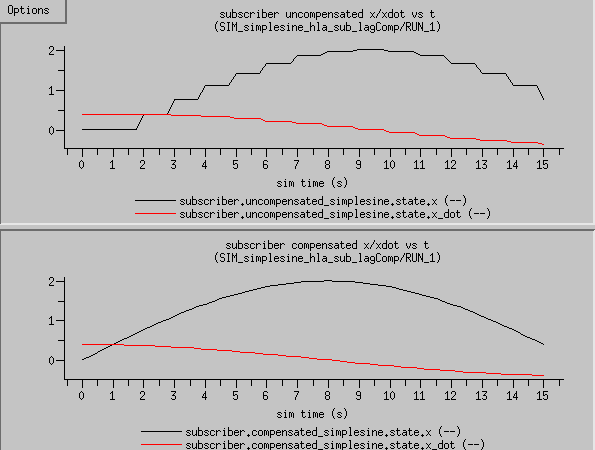
\includegraphics[width=4.5in]{TrickHLAUser-SIM-hla-sub-lagComp.png}
  \end{center}
\caption{Output from {\tt SIM\_simplesine\_hla\_sub\_lagComp}}
\label{fig:hla-sub-lagComp-output}
\end{figure}

\clearpage
